\section{AMP: Adversarial Model Perturbation}

\begin{frame}{From Empirical Risk to AMP Loss}

\begin{columns}

\column{0.66\textwidth}

In this paper, we optimize an alternative ``AMP loss''.

\vspace{1em}

\begin{equation*}
\mathcal{L}_\mathrm{ERM}(\boldsymbol{\theta}):=\frac{1}{|D|}\sum_{(\boldsymbol{x},\boldsymbol{y})\in\mathcal{D}}\ell(\boldsymbol{x},\boldsymbol{y};\boldsymbol{\theta})
\end{equation*}

\vspace{1em}

\begin{equation*}
\mathcal{L}_\mathrm{AMP}(\boldsymbol{\theta}):=\max_{\Delta:\Vert\Delta\Vert\le\epsilon}\mathcal{L}_\mathrm{ERM}(\boldsymbol{\theta}+\Delta)
\end{equation*}

\vspace{2em}

\column{0.34\textwidth}

\begin{figure}
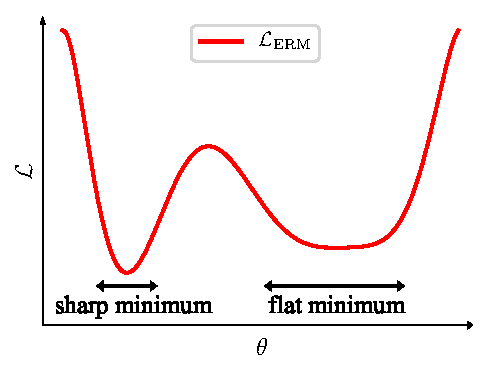
\includegraphics[width=.8\textwidth]{figs/loss_example_a.pdf}
\end{figure}
\vspace{-1.5em}
\begin{figure}
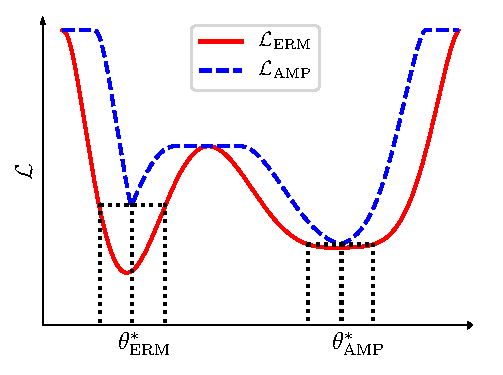
\includegraphics[width=.8\textwidth]{figs/loss_example_b.pdf}
\end{figure}
\end{columns}

\vspace{2em}

\end{frame}


\begin{frame}{Training Algorithm}

A mini-batch SGD is used for solving the ``min-max'' problem.

\vspace{-0.5em}

\begin{equation*}
\min_{\boldsymbol{\theta}}\max_{\Delta:\Vert\Delta\Vert\le\epsilon}\mathcal{L}_\mathrm{ERM}(\boldsymbol{\theta}+\Delta)
\end{equation*}

\begin{algorithm}[H]
\SetAlgoVlined
\While{$\boldsymbol{\theta}$ not converged}{
Initialize perturbation $\Delta$ with $\boldsymbol{0}$\;
\For{$n\gets1\text{ to }N$}{
Update $\Delta$ to maximize $\!\mathcal{L}_\mathrm{ERM}(\boldsymbol{\theta}\!+\!\Delta)\!$ via gradient ascent with learning rate $\zeta$\;
\If{$\Vert\Delta\Vert_2>\epsilon$}{
Normalize $\Delta$ to restrict its norm $\Vert\Delta\Vert_2$ to $\epsilon$;
}
}
Update $\boldsymbol{\theta}$ to minimize $\mathcal{L}_\mathrm{ERM}(\boldsymbol{\theta}\!+\!\Delta)$ via gradient descent with learning rate $\eta$\;
}
\caption{Adversarial Model Perturbation Training}
\end{algorithm}

\vspace{1em}

\end{frame}

\begin{frame}[fragile]{Implementation}
Source code: \url{https://github.com/hiyouga/AMP-Regularizer}

\begin{minted}[linenos]{python}
from amp import AMP
optimizer = AMP(model.parameters(), lr=0.1, epsilon=0.5, momentum=0.9)
for inputs, targets in dataset:
    def closure():
        optimizer.zero_grad()
        outputs = model(inputs)
        loss = loss_fn(outputs, targets)
        loss.backward()
        return outputs, loss
    outputs, loss = optimizer.step(closure)
\end{minted}
\end{frame}
